\section{Verbale della riunione}
	\subsection{Discussione punti emersi nell'ultimo confronto con il proponente}
	\begin{itemize}
		\item Ricevuta risposta sul parere del proponente riguardo i casi d'uso;
			\begin{itemize}
				\item {UC3.2: }Elimina utente -> attenzione a cosa può succedere se l'utente è in uso in quel momento;
				\item {UC4.2: }Inserimento priorità e modifica, la priorità conviene sia puramente numerica, per le modifiche conviene sempre lavorare nell'aggiungere le precondizioni in cui la modifica viene accettata.
			\end{itemize}
		\item Condivisione repository di GitHub ThreeWayMilkShake con il proponente;
		\item Fissato prossimo meeting su Google Meet con il proponente.
	\end{itemize}

	\subsection{Ricevimento con Prof. Cardin sui casi d'uso}
	Dopo il ricevimento con il docente Cardin sono emersi vari problemi da risolvere sui casi d'uso, e dunque sull'Analisi dei Requisiti in generale.
	\begin{enumerate}
		\item Caso d'Uso 1 (UC1 - Login):
			\begin{itemize}
				\item Modifica da "numero matricola operatore" a coppia username - password;
				\item Password auto generata, possibile cambio password chiedendo ad admin.
			\end{itemize}
		\item Uso delle inclusioni errate nei casi d'uso:
			\begin{itemize}
				\item Uso delle inclusioni per modellare quanto dovrebbe essere stato modellato con sotto-casi d'uso;
				\item Non c'è un prima e un dopo nei diagrammi, inclusione ha una sequenzialità;
				\item Nei casi d'uso 4.2 e 4.3 abbiamo sbagliato, li abbiamo trattati come inclusioni, quando avrebbero dovuto essere 4.1.1 e 4.1.2;
				\item Nei casi d'uso 8.1 e 8.2 abbiamo usato inclusioni, quando in realtà sono generalizzazioni di 8.
			\end{itemize}
		\item Utilizzato impropriamente le relazioni di ereditarietà:
			\begin{itemize}
				\item Casi d'uso UC7.2 e 7.3 e 7.4 sono sotto-casi d'uso di 7.1, quindi diventano 7.1.1, 7.1.2, 7.1.3 e 7.1.4.
			\end{itemize}
		\item Rivedere i requisiti di vincolo, molti sono requisiti funzionali;
		\pagebreak
		\item I diagrammi di attività hanno numerosi errori di sintassi UML.
		\begin{center}
			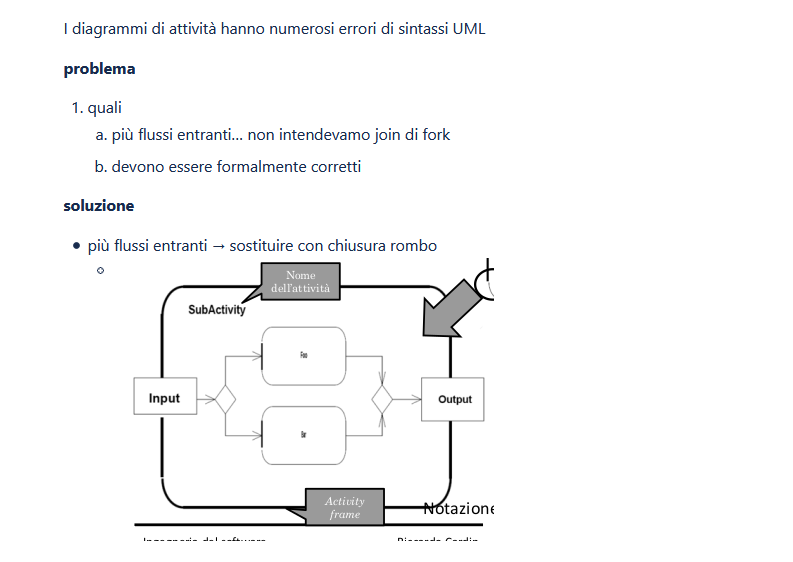
\includegraphics[scale=0.8]{cardin_1}\\
		\end{center}
	\end{enumerate}
	\pagebreak
	\subsection{Discussione sul PoC}
	Il PoC (Proof of Concept) deve comprendere:
	\begin{itemize}
		\item funzionalità che ci permettano di implementare più tecnologie possibili;
		\item mostrare che abbiamo compreso le tecnologie;
		\item integrare il più possibile le tecnologie.
	\end{itemize}

    \noindent Il PoC (Proof of Concept) deve comprendere:
    \begin{itemize}
        \item funzionalità che ci permettano di implementare più tecnologie possibili;
        \item mostrare che abbiamo compreso le tecnologie;
        \item integrare il più possibile le tecnologie.
    \end{itemize}




